% A degreewise splitting of cycles from a finite free chain complex over a PID.
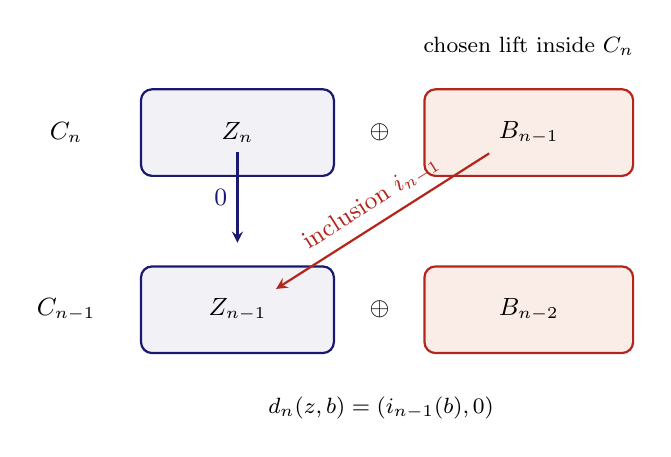
\begin{tikzpicture}[font=\small,>=stealth,x=1cm,y=1cm]
\node at (-1.3,2.25) {$C_n$};
\node at (-1.3,0) {$C_{n-1}$};
\draw[rounded corners,thick,MidnightBlue,fill=MidnightBlue!6] (-0.35,1.7) rectangle (2.1,2.8);
\draw[rounded corners,thick,BrickRed,fill=BrickRed!6] (3.25,1.7) rectangle (5.9,2.8);
\node (zn) at (0.875,2.25) {$Z_n$};
\node at (2.68,2.25) {$\oplus$};
\node (bn) at (4.575,2.25) {$B_{n-1}$};
\draw[rounded corners,thick,MidnightBlue,fill=MidnightBlue!6] (-0.35,-0.55) rectangle (2.1,0.55);
\draw[rounded corners,thick,BrickRed,fill=BrickRed!6] (3.25,-0.55) rectangle (5.9,0.55);
\node (znm) at (0.875,0) {$Z_{n-1}$};
\node at (2.68,0) {$\oplus$};
\node (bnm) at (4.575,0) {$B_{n-2}$};
\draw[->,thick,BrickRed] (bn.south west) -- node[above,sloped] {inclusion $i_{n-1}$} (znm.north east);
\draw[->,thick,MidnightBlue] (zn.south) -- node[left] {$0$} (0.875,0.85);
\node[font=\footnotesize,align=center] at (4.575,3.35) {chosen lift inside $C_n$};
\node[font=\footnotesize,align=center] at (2.7,-1.25) {$d_n(z,b)=(i_{n-1}(b),0)$};
\end{tikzpicture}
